\documentclass[main.tex]{subfiles} 
\begin{document}

\section*{Teoretisk bakgrunn}

\begin{figure}[h!]
\centering
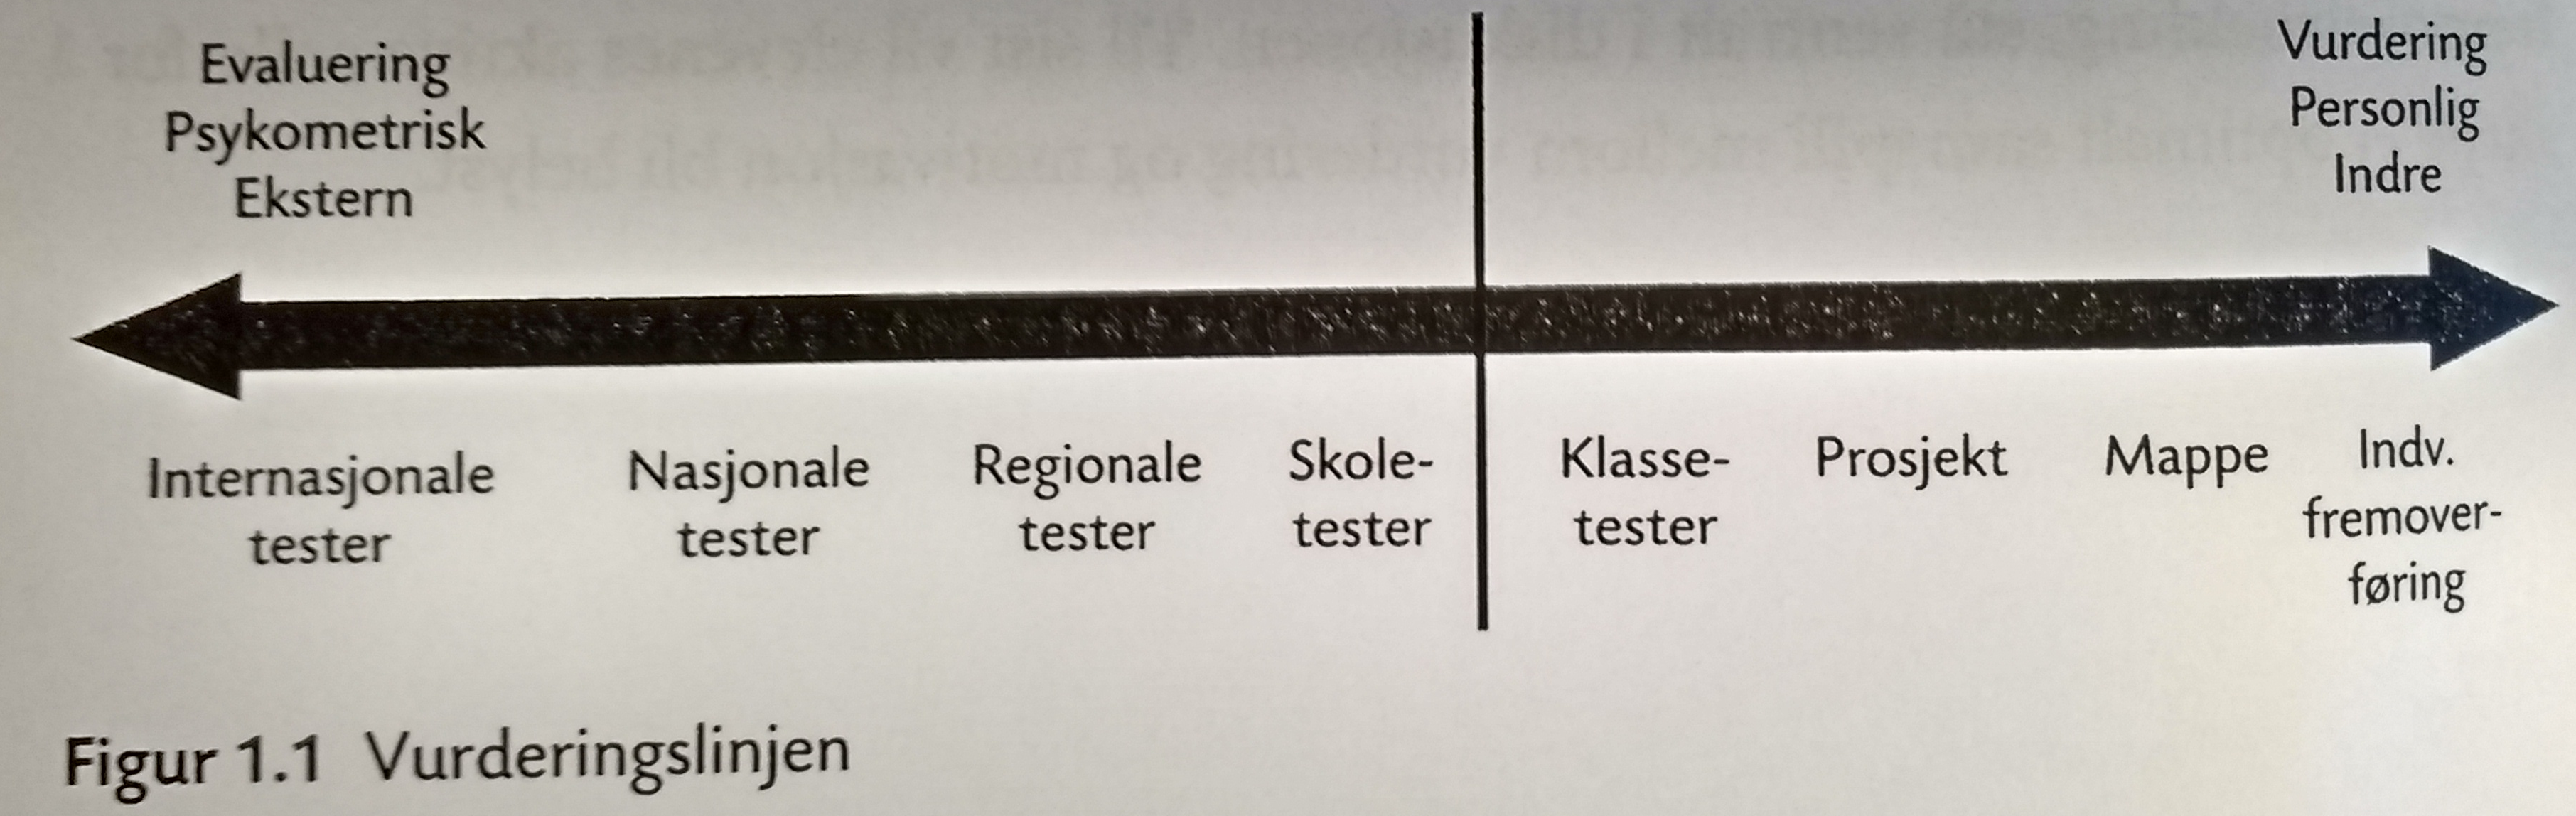
\includegraphics[scale = 0.1]{../figures/vurderingslinjen.png}
\caption{Vurderingslinjen. Kilde: \protect\citeA{smit09}.}
\label{fig:smit09}
\end{figure}

\citeA[s. 3]{smit09} beskriver hvordan vurderingslandskapet forandrer seg, fra internasjonale tester til
individuell fremoverføring. Gjennom \emph{vurderingslinjen} (se figur \ref{fig:smit09}) beskriver hun
hvordan informasjonen går fra å evaluere en nasjon i forhold til andre nasjoner, skoler i distrikter, 
og til slutt på lokalt nivå fra klasser i skolen til enkelt elever i en klasse. Ofte vil politiske styringsorganer
befinne seg på venstre siden av vurderingslinjen, og lærere og elever på høyre siden. Men tiltross for det, 
for undervisere er det viktig å ha oversikt over internasjonale resultater, gjennom f.eks. PISA 
undersøkelsen\footnote{I  PISA-undersøkelsen blir norske 15-åringer sammenliknet med jevnaldrende ungdommer i 
andre OECD-land innen tre sentrale kompetanseområder: matematikk, lesing og naturfag.}. 
Her kan resultatene ha noe å si om hvordan elevenes prestasjoner i ulike fagområder henger sammen med ulike 
bakgrunnsvariabler (\citeNP[s. 11]{klor04}). 

En annen undersøkelse, TIMMS, brukes til å evaluere elever helt fra 4.trinn
til andre året på videregående skole. Metastudiet (\citeNP{grol06}) baserer seg på resultater fra både TIMMS og PISA. 
Forskerne Grønmo og Olsen, skriver blant annet at det er interessant å merke forskjellene i resultatene mellom disse to 
studiene. Mens PISA fokuserer på oppgaver rettet nærmere mot virkeligheten, med tabeller og figurer tatt fra virkelige
kontekster, har TIMMS større fokus på ren matematikk. Studiet konkluderer med, for at elevene skal gjøre det bedre
i anvendt matematikk, trenger de en solid fundament i grunnleggende ferdigheter, deriblant tall og tallforståelse 
(\citeNP{grol06}). Dette har også jeg selv observert gjennom karleggingsprøven. Det var spesielt i oppgave 2.b 
(se vedlegg 1) at elevenes svakheter i tallforståelse kom tydelig fram.

For eleven derimot er det endatil viktigere å ha informasjon om egen læringsprosess, og denne informasjonen er kritisk 
for en lærer for å vurdere sin egen undervisningspraksis. I læringsrettet vurdering stilles det strengere krav til 
lærerers evner som evaluator. Holdning til vurdering forandrer fra en læringsteori til en annen. Det kan være 
interessant å se på lærerens læringssyn. Her er følger to eksempeler på forskjellige læringssyn.

\subsection*{Læring som overføring av kunnskap eller en relasjonell prosess}

I behavioristisk læringsteori foregår læring ved overføring av kunnskap, uavhengig av relasjonen mellom lærer 
og elev. Elev blir anskuet som et tomt kar, som det er lærerens jobb å fylle med kunnsakp. 
I et slikt læringssyn er vurdering i seg selv relativt ukomplisert, siden da gjelder det å 
formulere sine tilbakemeldinger på en så presis og elevtilpasset måte som mulig.
Derimot forventes det da at eleven tar til seg tilbakemeldingene og bruker dem til å rette seg etter.
Tilbakemeldingene vil da være begrenset til spesifikke svakheter relatert til faget eller kompetansemål.
I artikelen \citeA[s.431]{foss14}, skriver hun at utstrakt bruk av individuell veiledning kan føre
til manglende inkludering. Siden individualiserte metoder krever stor selvstendighet hos elevene, vil
elever som har vansker med selvregulært læring falle utenfor. Videre er betinging sentralt i behaviorismens 
syn på læring (\citeNP[s. 74]{salj13}). Ved ønsket atferd belønnes handlingen. Dette referes som forsterking 
(\citeNP[s. 22]{hell07}). Innenfor vurderingskontekten er hensikten å motivere elevene. Dermed er karakteren en 
forsterker for noen og straff for andre. Gjennom egen praksis, både som observatør og sensor i muntlig eksamen,
har jeg sett at for noen elever kan karakterer være både motiverende og en drivkraft i seg selv. Derimot
har jeg også observert at det kan ha en ødeleggende effekt. Smith skriver at det ligger innenfor
lærerens profesjonelle ansvar å prøve å komme frem til det optimale sampillet mellom vurdering og 
motivasjon (\citeNP[s. 23]{smit09}).

Så hva er problemet med en behavioristisk tilnærming til vurdering for læring? La oss tenke at klasserom er 
et sted hvor alle elever er tilnærmet like i hvordan de oppfatter matematikk og hvor deres vanskeligheter ligger. 
Da er det selvfølgelig helt kurant å lage tydelige skriftlige tilbakemeldinger og fremovermeldinger, i et format 
som passer for hele klassen. Dessverre så finnes det ikke slike klasserom, med mindre elever er oppdelt etter nivå. 
Permanent nivådelt undervisning strider mot det overordnede prinsippet tilpasset opplæring (\citeNP[s. 426]{foss14}). 
Fosse kaller dette for organisatorisk differensiering:
\begin{displayquote}
\textelp{}. Til vanlig skal organisering ikke skje etter faglig nivå, kjønn eller etnisk tilhørlighet. (Opplæringsloven)
\end{displayquote}
Hun referer til metastudie (\citeNP{hatt09}) når hun skriver at de flinke elevene kan dra nytte av organisatorisk
differensiert undervisning, men det har ikke ønsket effekt for elever som strever med faget (\citeNP[s. 423]{foss14};
\citeNP[s. 168]{olma15}). 
Ifølge opplæringsloven skal alle elever få en opplæring tilpasset etter deres evner og forutsetninger. Et annet problem 
med en slik tilnærming er at elevens deltagelse i egen utvikling blir fraværende i et slikt rigid system. Siden eleven er 
kun en mottager, kan eleven ikke være med og aktivt delta i egen vurdering. 
\newline

Sett fra det relasjonelle perspektivet i sosiokulturell teori, består det i å veilede elevene i den 
nærmeste utviklingssonen. Den \emph{nærmeste utviklingssonen} beskriver en sone som ligger i mellom en elevs kognitive 
ferdigheter, dvs. hva de kan oppnå selvstendig uten hjelp, og elevens potensielle utvikling, dvs. 
hva en elev kan få til eller forstå gjennom veiledning (\citeNP[s. 125]{bta98}; \citeNP[s. 75]{salj13}). 
Bruk av ''scaffolding`` eller stillasbygging (\citeNP{bta98}) er da viktig for å knytte fagbegreper og 
teori til elevenes forkunnskaper. Vurderingsarbeidet vil derfor også gi den forskende lærer (\citeNP[s. 19]{hell07}) 
verdifull informasjon om sin egen didaktiske tilrettelegging. Gjennom f.eks. elevsamtale kan elev ikke bare få 
tilbakemelding om hvor hen står faglig, men også gi veiledning som kan hjelpe eleven videre i faglig utvikling.
Ifølge \citeA[s.96]{tang10} vil da elevsamtalen være en form for formativ evaluering.

En av sentrale styringsrammene for norsk utdanningspolitikk og skolepraksis er prinsippet om tilpasset opplæring.
Opplæringen skal ivareta sentrale verdier som inkludering, variasjon, sammenheng, relevans, verdsetting, medvirkning og 
erfaringer. Dette skal operasjonaliseres av undervisere gjennom differensiering (\citeNP[s. 169]{olma15}).
Undervisningen må, ved hjelp av differensiering, tilfredsstille alle elevenes tilretteleggingsbehov i klassen, fra 
elever med matematikkvansker (dyskalkuli) til evnerike elever. Når en lærer jobber med elever hvor spennet er så 
pass stort, med andre ord at elevene utgjør en heterogen gruppe, da kan heller ikke undervisningen være homogenisert. 
\begin{displayquote}
Tilpasset opplæring innebærer at læreren kjenner til, utnytter og legger til rette for at eleven kan utnytte
sine læringsstrategier, formativ elevvurdering innebærer at læreren veileder det videre arbeidet mot høyere måloppnåelse,
bl.a. med utgangspunkt i elevens  bruk av læringsstrategier.
(\citeNP[s. 162]{engh11}) 
\end{displayquote}
Jeg kan derfor allerede nå påstå 
at en behavioristisk tilnærming til vurdering for læring vil tydeligvis ikke oppfylle prinsippet om tilpasset opplæring.

Videre nå vil jeg gjennomgå bakgrunn for kartleggingsprøven, deretter vil jeg oppsummere gjennomføringen og resultatene.
Disse resultatene vil jeg drøfte i lys av pedagogisk og fagdidaktisk teori, og tilslutt vil jeg se hvordan jeg 
kan bruke dette videre i mitt undervisningsarbeid. 



\end{document}
